\scanpage{26}
Soit $X$ un ens. Une \uline{décomposition binaire} de $X$ est un ens de deux parties de $X$ $(\Sigma_{\alpha}^{\alpha})_{\alpha\in\unsure{\mathcal E|\mathscr E|\varepsilon}}$ (les ``hémisphères'') dont la réunion est $X$, et dont \deleted{l'intersection} aucune n'est contenue dans l'autre -- on désigne par $E$ (``équateur'') l'intersection (on n'exclut pas qu'elle soit vide). Quand $X$ est un espace topologique, on s'intéresse au cas où les hémisphères $\Sigma_{\alpha}$ sont fermés, (et \inserted{de} plus, le plus souvent, \inserted{$\Sigma_{\alpha}^{\alpha}$ et $\Sigma_{\deleted{\unsure{\alpha}}}^{\alpha}\setminus E=\Sigma_{\deleted{\unsure{\alpha}}}^{\deleted{\unsure{\alpha}}\alpha,\unsure{0|\circ|o}}$} connexes \deleted{\unsure{$\Sigma_{\alpha}$|les}} et où $E\ne\varnothing$); si les $\Sigma_{\deleted{\unsure{\alpha}}}^{\alpha}$ connexes et $E\mathrel{\unsure{\ne|+}}\varnothing$, $X$ est connexe, si \deleted{les $\Sigma_{\alpha}^{\alpha,0}$ connexes}, \inserted{$X$ connexe, \deleted{et}} on conclut \unsure{\deleted{aussitôt}} que $\overline{\Sigma^{\alpha,0}}\cap E\ne\varnothing$
% margin note written sideways
\reversemarginpar\margin{\figure{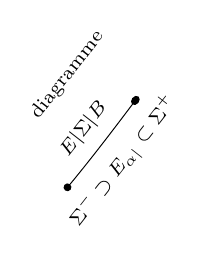
\begin{tikzpicture}[x=1mm,y=1mm,line cap=round,line join=round,font=\scriptsize]
\begin{scope}[rotate=52,transform shape]
\draw[line width=.35pt] (0,0) .. controls (4.6,-.15) and (9.5,-.08) .. (14,0);
\fill (0,0) circle[radius=.5mm];
\fill (14,0) ellipse[x radius=.64mm,y radius=.49mm];
\node[anchor=base west,inner sep=0pt] at (4.4,8.2) {diagramme};
\node[inner sep=0pt] at (7.1,2.9) {$\deleted{\unsure{E|\Sigma|B}}$};
\node[inner sep=0pt] at (7,-3.6) {$\Sigma^{-}\supset E_{\unsure{\alpha|{}}}\subset\Sigma^{+}$};
\end{scope}
\end{tikzpicture}}}\normalmarginpar
(car $\overline{\Sigma^{\alpha,0}}\cap E=\overline{\Sigma^{\alpha,0}}\setminus\Sigma^{\alpha,0}$, et $\Sigma^{\alpha,0}$ ne peut être à la fois ouvert et fermé car $\Sigma^{\unsure{-,0|\alpha,0|-\alpha,0}}$, est un ouvert $\ne\varnothing$ et $\ne X$)

Considérons deux décompositions binaires $\{\Sigma_1^{+},\Sigma_1^{-}\},\unsure{[|(}\Sigma_2^{+},\Sigma_2^{-}\}$ \deleted{\unsure{distinctes}} \inserted{de $X$,} on dit qu'elles sont \uline{\unsure{non panachées|non penchées|non parallèles|en position}} si \inserted{elles sont \uline{distinctes}, et si} on peut trouver $\Sigma_1^{+}$ dans l'une, $\Sigma_2^{+}$ dans l'autre, tels que
\[
\Sigma_1^{+}\cap\Sigma_2^{+}=\varnothing\qquad(\text{d'où }E_1\cap E_2=\varnothing)
\]
on \unsure{a} alors
\[
\begin{aligned}
\Sigma_1^{+}&\mathrel{\unsure{\deleted{\cap}\subset|\subset}}\Sigma_2^{-}\ \deleted{\ne\varnothing}\quad\text{i.e.}\quad\Sigma_1^{+}\cap\Sigma_2^{-}=\Sigma_1^{+}\\
\Sigma_2^{+}&\subset\Sigma_1^{-}\qquad\qquad\text{\unsure{i.e.|ie}}\quad\Sigma_2^{+}\cap\Sigma_1^{-}=\Sigma_2^{+}\\
\Sigma_{12}&\overset{\text{déf}}{=}\Sigma_1^{-}\cap\Sigma_2^{-}\supset E_1\cup E_2,\quad\Sigma_1^{-}\cap\Sigma_2^{-}\ne\varnothing
\end{aligned}
\]
% archive sheet number: 25
